% ============================================================
%  Towards FPGA Acceleration of STDP-Based Neural Simulation
%  Short paper -- 5 pages max
% ============================================================
\documentclass[10pt,twocolumn]{article}

% --- Packages ---
\usepackage[T1]{fontenc}
\usepackage[utf8]{inputenc}
\usepackage{lmodern}
\usepackage{textcomp}
\usepackage[margin=1.8cm, top=2.0cm, bottom=2.0cm]{geometry}
\usepackage{graphicx}
\usepackage{amsmath,amssymb}
\usepackage{booktabs}
\usepackage{caption}
\usepackage{subcaption}
\usepackage{microtype}
\usepackage{hyperref}
\usepackage{cite}
\usepackage{xcolor}

\captionsetup{font=small, labelfont=bf, skip=4pt}
\setlength{\columnsep}{0.5cm}

% Title block
\title{%
  \textbf{Quantifying the Computational Cost of STDP in Spiking\\
  Neural Networks: A Benchmark Study Towards FPGA Acceleration}
}
\author{%
  Maxime Carriere$^{1}$\\
  \small $^{1}$\,Brain Language Laboratory, Freie Universit\"{a}t Berlin\\
  \small \texttt{maxime.carriere@fu-berlin.de}
}
\date{\small March 2026 --- Preliminary results}

% ============================================================
\begin{document}
\maketitle
\thispagestyle{empty}

% ============================================================
\begin{abstract}
Spiking Neural Networks (SNNs) trained with Spike-Timing Dependent
Plasticity (STDP) offer a biologically plausible model of learning.
Their simulation, however, carries a heavy computational cost that
grows super-linearly with network size.
Using the NEST simulator across 2\,160 configurations
(network size, connection density, firing rate, and core count),
we show that STDP can more than \emph{double} total simulation time
compared to static synapses---an overhead reaching 183\%
for networks of 8\,000 neurons.
Multi-core CPU parallelism scales both synaptic rules equally but
cannot close the STDP overhead gap: STDP remains $\sim\!2\times$
slower than static at all core counts.
These findings motivate a hardware-accelerated solution.
We present these benchmarks as a foundation for designing an
FPGA-based STDP co-processor.
\end{abstract}

% ============================================================
\section{Introduction}
\label{sec:intro}

The human brain processes sensory information and learns from
experience using approximately $10^{11}$ neurons connected by
roughly $10^{15}$ synapses \cite{azevedo2009}.
Unlike the artificial neural networks behind today's deep-learning
revolution---which use smooth continuous activations and
gradient-based training—biological neurons communicate through
discrete electrical pulses called \emph{spikes}.
Models that respect this mechanism are called \emph{Spiking Neural
Networks} (SNNs).

SNNs are of great interest for neuromorphic computing, low-power
embedded intelligence, and fundamental neuroscience research.
However, simulating even a small fraction of biological-scale
networks on conventional computers remains extremely expensive.
A key bottleneck is the learning rule that governs how synaptic
connections are updated during simulation.

In this work we focus on the dominant biological learning rule:
\textbf{Spike-Timing Dependent Plasticity} (STDP).
We systematically benchmark its computational overhead using the
widely used \emph{NEST} simulator \cite{gewaltig2007}
and identify the scaling regimes where conventional CPUs become
inadequate.
Our ultimate goal is to offload STDP weight updates to an
FPGA co-processor, enabling real-time simulation of large networks
at a fraction of the energy cost.

% ============================================================
\section{Background: What is STDP?}
\label{sec:stdp}

\subsection{Synaptic plasticity}

Learning in biological neural circuits is implemented by changing
the \emph{strength} (weight) of synaptic connections.
A synapse connects a \emph{pre-synaptic} neuron
(the one sending a signal) to a \emph{post-synaptic} neuron
(the one receiving it).
The key insight from Hebbian theory is:
\emph{neurons that fire together wire together} \cite{hebb1949}.

\subsection{The STDP rule}

STDP refines this idea by making the weight change depend on the
\emph{relative timing} of the two spikes, as first demonstrated
experimentally by Markram et al.\ \cite{markram1997} and
subsequently characterised in hippocampal neurons by
Bi and Poo \cite{bi1998}.
Define $\Delta t = t_{\text{post}} - t_{\text{pre}}$,
the interval between the post-synaptic and pre-synaptic spike.
The weight update follows an exponential learning window
(Fig.~\ref{fig:stdp}):

\begin{equation}
  \Delta W =
  \begin{cases}
    A_+ \, e^{-\Delta t / \tau_+} & \text{if } \Delta t \geq 0 \quad \text{(LTP)}\\
    -A_- \, e^{+\Delta t / \tau_-} & \text{if } \Delta t <  0 \quad \text{(LTD)}
  \end{cases}
  \label{eq:stdp}
\end{equation}

\noindent where $A_{\pm}$ are the learning rates and $\tau_{\pm}$ are
time constants (typically $\approx 20$\,ms).
When the pre-synaptic neuron fires \emph{before} the post-synaptic
one ($\Delta t > 0$), the synapse is \emph{strengthened}
(Long-Term Potentiation, LTP).
In the opposite case it is \emph{weakened}
(Long-Term Depression, LTD).
This biologically observed rule is illustrated in
Fig.~\ref{fig:stdp}.

\begin{figure}[h]
  \centering
  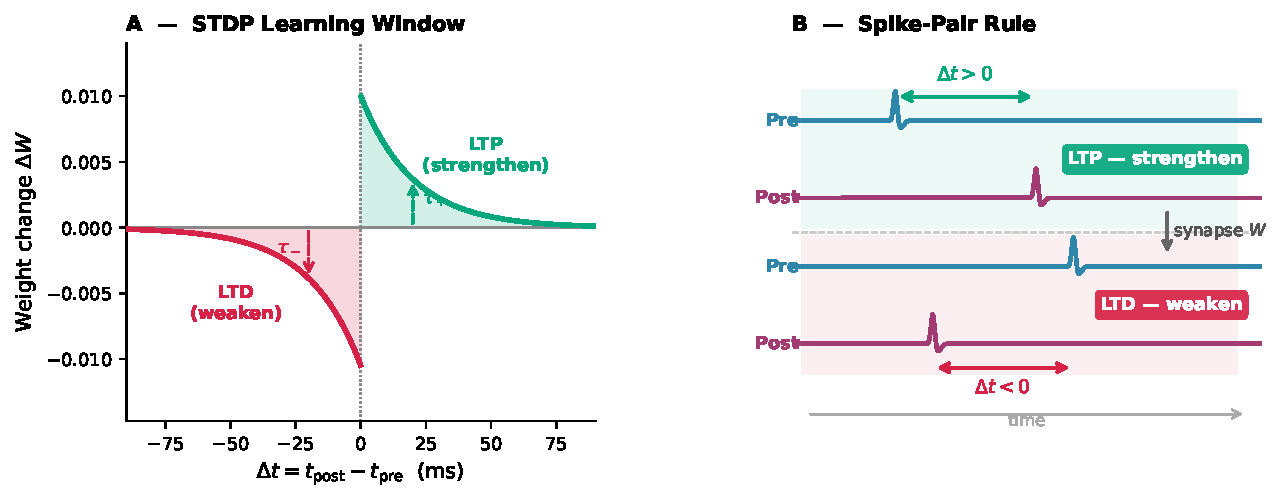
\includegraphics[width=\linewidth]{figures/paper_fig1_stdp_intro.pdf}
  \caption{%
    \textbf{STDP learning window.}
    \textbf{(A)} Weight change $\Delta W$ as a function of the
    inter-spike interval $\Delta t$ (Eq.~\ref{eq:stdp}).
    Pre fires before post ($\Delta t > 0$): synapse strengthens (LTP,
    green).
    Post fires before pre ($\Delta t < 0$): synapse weakens (LTD, red).
    \textbf{(B)} Schematic of a spike pair.
    The synapse weight $W$ is updated after every spike pair
    according to their relative timing.
  }
  \label{fig:stdp}
\end{figure}

\subsection{Computational cost of STDP}

For a network of $N$ neurons with $S$ synapses, every spike triggers
a weight update at each affected synapse.
The total number of operations per second scales as:
\[
  \text{Updates/s} \;=\; \nu \cdot N \cdot \bar{k}
\]
where $\nu$ is the mean firing rate and $\bar{k}$ is the mean
in-degree (number of incoming synapses per neuron).
With $N\!=\!2\,000$, $\nu\!=\!20$\,Hz, and $p_{\rm conn}\!=\!0.1$,
this yields $\approx\!8 \times 10^6$ updates per second---all of which
must be serialised on a CPU, incurring memory-bandwidth pressure and
branch-prediction penalties that grow super-linearly with $N$
(as shown below),
as shown below.

% ============================================================
\section{Experimental Setup}
\label{sec:methods}

We used \textbf{NEST 3.6} \cite{gewaltig2007} to simulate recurrent
networks of \texttt{iaf\_psc\_alpha} integrate-and-fire neurons
driven by Poisson external input.
Each configuration was simulated for 20\,s of biological time.
The parameter space covered:

\begin{itemize}\setlength\itemsep{0pt}
  \item Network size $N$: 10 to 16\,000 neurons (10 values)
  \item CPU cores: 1, 2, 4, 8
  \item Connection probability $p$: 5\%, 10\%, 20\%
  \item External firing rate: 10, 20, 40\,Hz
  \item Learning rule: \emph{static synapses} vs. \emph{additive STDP}
        ($\tau_{\pm}\!=\!20$\,ms, $\lambda\!=\!0.01$)
\end{itemize}

In total, 2\,160 simulations were run (3 trials each for statistical
error bars), collected over 2.9 days on a standard desktop workstation
running Arch Linux.
Timing was measured with \texttt{time.perf\_counter()},
separating the network \emph{setup} phase from the
\emph{simulation} phase.
All data and scripts are available on request.

% ============================================================
\section{Results}
\label{sec:results}

\subsection{STDP overhead is negligible below 1\,000 neurons,
then becomes critical}

Fig.~\ref{fig:timing} compares simulation time for static and STDP
networks as a function of network size, at 1 core, $p\!=\!0.1$,
and 20\,Hz.
For small networks ($N \leq 500$) the overhead is negligible:
both rules complete in under 5\,s and the bars are nearly identical
(Fig.~\ref{fig:timing}A).
The linear-scale plot in Fig.~\ref{fig:timing}B reveals a sharp
transition around $N\!\approx\!1\,000$ neurons, above which the two
curves diverge dramatically.
At $N\!=\!2\,000$ STDP takes $1.9\times$ longer (53\,s vs.\ 28\,s);
at $N\!=\!4\,000$ it reaches $2.3\times$ (177\,s vs.\ 76\,s);
and at $N\!=\!8\,000$ it takes $2.4\times$ longer
(808\,s vs.\ 330\,s)---an absolute overhead of nearly
\textbf{8 minutes per simulation}.

\begin{figure}[h]
  \centering
  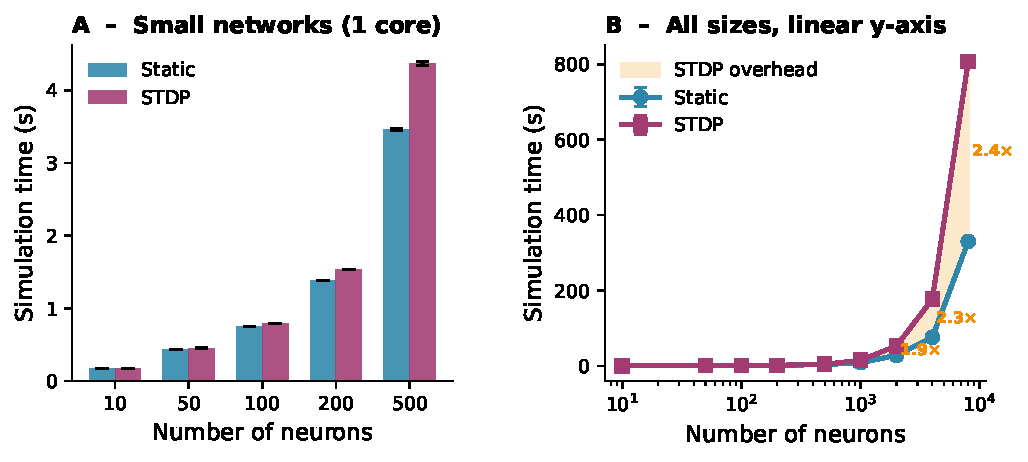
\includegraphics[width=\linewidth]{figures/paper_fig2_simple_timing.pdf}
  \caption{%
    \textbf{Static vs.\ STDP simulation time.}
    \textbf{(A)} Bar chart for small networks.
    \textbf{(B)} Full log-scale comparison; shaded region marks the
    STDP overhead.
    Each point is the mean of 3 trials; error bars show SEM.
    Conditions: 1 core, $p\!=\!0.1$, 20\,Hz Poisson input.
  }
  \label{fig:timing}
\end{figure}

\subsection{Overhead peaks around 4\,000 neurons then partially
stabilises}

Fig.~\ref{fig:overhead}A shows the STDP overhead (relative to
static, \%) as a function of $N$ for three connection densities.
For $p\!=\!0.1$ the overhead is below 5\% up to $N\!=\!100$,
then rises steeply, exceeding \textbf{50\%} at $N\!\approx\!500$
and surpassing \textbf{100\%} at $N\!\approx\!1\,000$.
The maximum recorded overhead is $\mathbf{183\%}$ at
$N\!=\!4\,000$ ($p\!=\!0.2$, 10\,Hz): a 183\% overhead means
STDP takes $2.83\times$ \emph{as long} as the static baseline
(total$\,=\,$static$\,+\,$183\%$\,\times\,$static).
Note that at the highest firing rate (40\,Hz) and density
($p\!=\!0.2$), the percentage overhead \emph{decreases} for the
largest networks because the static simulation itself becomes
expensive; however, the absolute overhead remains hundreds of
seconds.

Fig.~\ref{fig:overhead}B plots the STDP overhead \emph{per synapse}.
Rather than staying constant (ideal dashed line), the cost per
synapse increases with $N$, revealing super-linear behaviour.
The bottleneck is not the update arithmetic itself, but
memory-access patterns: as the synapse table outgrows the CPU cache,
cache misses accumulate and per-update cost rises.

\begin{figure}[h]
  \centering
  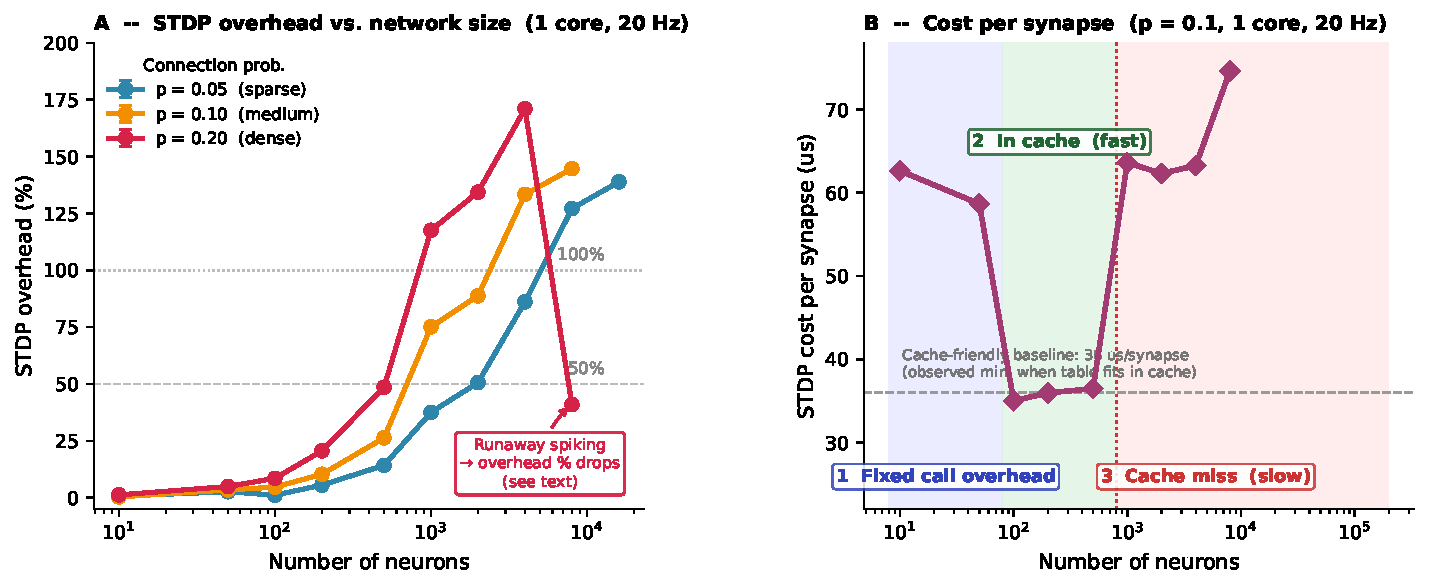
\includegraphics[width=\linewidth]{figures/paper_fig3_overhead_scaling.pdf}
  \caption{%
    \textbf{STDP overhead scaling.}
    \textbf{(A)} Percentage overhead vs.\ network size for three
    connection probabilities (1 core, 20\,Hz).
    Dashed lines mark 50\% and 100\% overhead thresholds.
    \textbf{(B)} STDP overhead per synapse; the non-flat curve
    reveals super-linear scaling due to memory-access pressure.
  }
  \label{fig:overhead}
\end{figure}

\subsection{Multi-core parallelism does not close the STDP gap}

A natural first response to the STDP overhead is to simply use more
CPU cores: if STDP doubles the computation, perhaps running on two
cores restores the original speed.
Fig.~\ref{fig:multicore} tests this intuition directly.

\textbf{Speedup with more cores (Panel A).}
For static synapses, parallelism is beneficial only for large
networks.
Below $N\!=\!500$ neurons, adding cores barely helps or even hurts
performance: coordinating multiple threads requires constant
communication between them, and for small workloads this coordination
cost exceeds the time saved by splitting the work.
At 10 neurons, 8 cores are actually $1.8\times$ \emph{slower} than a
single core.
For large networks ($N \ge 2\,000$), multi-core scaling is
substantial, reaching close to or above the ideal linear line.
The practical ceiling for this hardware configuration sits around
$10\times$ speedup with 8 cores.

\textbf{The STDP overhead gap persists at every core count (Panel B).}
Panel B shows the raw wall-clock simulation time for both static and
STDP synapses at $N\!=\!4\,000$ neurons---the most informative way to
compare the two learning rules under parallelism.
Both curves decrease steeply as cores are added, confirming that
parallelism is effective for both rule types.
Going from 1 to 8 cores reduces static time from 76\,s to 7.8\,s
($9.7\times$ faster) and STDP time from 177\,s to 16\,s
($11.0\times$ faster).

Yet at every single core count, STDP remains approximately
$2.1$--$2.3\times$ slower than static, as shown by the bracket at 8
cores.
The two curves run in parallel: they drop at the same rate, keeping
the same proportional distance from each other.
This is the key finding---\textbf{adding more CPU cores cannot
eliminate the STDP overhead}.
Each core still has to execute the same weight-update calculation for
every synapse; parallelism simply divides this work among more
processors, but does not make the calculation itself any cheaper.

Think of it this way: if STDP requires ten steps where static
requires four, then splitting across eight cores gives you eight
workers each doing ten steps vs.\ four steps.
Every worker is still $2.5\times$ slower on their share of the work.
The ratio never changes.

This finding has an important practical implication.
Scaling from 1 to 8 cores on a typical server is already a
significant hardware investment.
Yet even with this investment, a biologically realistic network with
STDP synapses will always simulate $2\times$ slower than the same
network with fixed weights.
For real-time or near-real-time brain-computer interface applications,
this gap is unacceptable.
A fundamentally different solution is needed---one that reduces the
cost of the STDP computation itself rather than distributing it more
efficiently.

\begin{figure}[h]
  \centering
  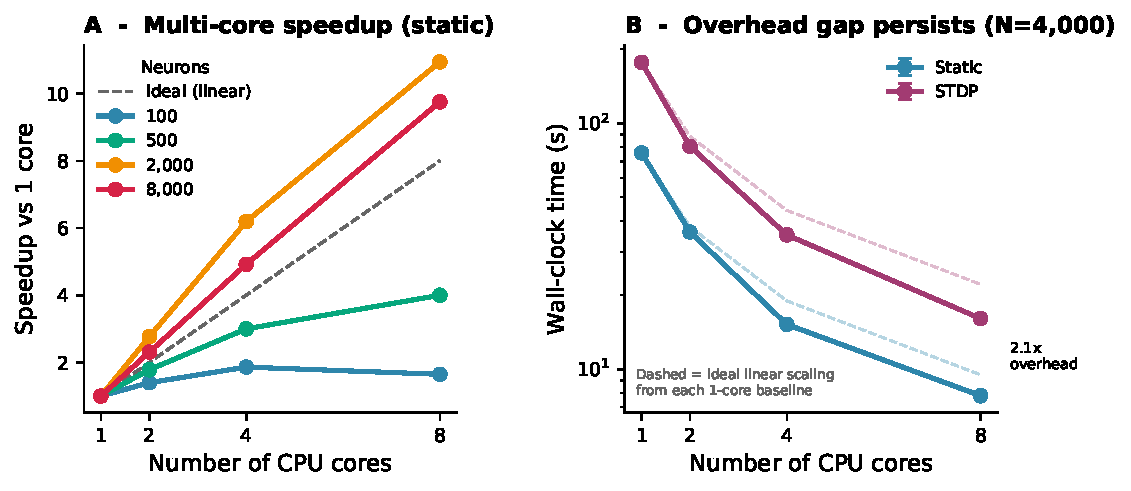
\includegraphics[width=\linewidth]{figures/paper_fig4_multicore.pdf}
  \caption{%
    \textbf{Multi-core scaling.}
    \textbf{(A)} Speedup relative to 1 core for different network
    sizes (static synapses, $p\!=\!0.1$, 20\,Hz); dashed line is
    ideal linear scaling.
    Small networks ($\le\!500$ neurons) gain little or nothing from
    additional cores.
    \textbf{(B)} Absolute wall-clock simulation time for static and
    STDP synapses at $N\!=\!4\,000$.
    Both rules scale similarly with core count (faint dashed lines
    show ideal scaling from each 1-core baseline), but the STDP
    overhead of $\sim\!2.1\times$ persists regardless of how many
    cores are used.
    More cores speed up both rules equally---they do not close
    the gap.
  }
  \label{fig:multicore}
\end{figure}

% ============================================================
\section{The Case for FPGA Acceleration}
\label{sec:fpga}

The results above identify a clear bottleneck:
STDP weight updates incur a super-linearly growing cost that
neither multi-core CPUs nor memory optimisation can fully address.
The root cause is architectural: a general-purpose CPU must

\begin{enumerate}\setlength\itemsep{0pt}
  \item \textbf{Fetch} the synapse record from DRAM (cache-miss prone),
  \item \textbf{Compute} the exponential decay $e^{-\Delta t/\tau}$,
  \item \textbf{Write back} the updated weight—millions of times
        per second.
\end{enumerate}

FPGAs (Field-Programmable Gate Arrays) offer a compelling alternative
because:
\begin{itemize}\setlength\itemsep{0pt}
  \item \textbf{Massive parallelism}: an FPGA can process hundreds of
        synaptic updates simultaneously in dedicated hardware lanes.
  \item \textbf{On-chip BRAM}: synapse tables for moderate networks
        fit in fast on-chip memory, eliminating DRAM latency.
  \item \textbf{Fixed-point exponentials}: the STDP kernel
        (Eq.~\ref{eq:stdp}) maps efficiently to lookup tables.
  \item \textbf{Energy efficiency}: FPGA implementations of neural
        simulation consume 10–100$\times$ less power than GPU or CPU
        equivalents \cite{cheung2012,han2020}.
  \item \textbf{Deterministic latency}: unlike CPUs, an FPGA pipeline
        has cycle-accurate timing, simplifying the spike-timestamp
        bookkeeping required by STDP.
\end{itemize}

Several FPGA-based SNN accelerators have been proposed
\cite{cheung2012,sripad2020,han2020}, but none directly targets the
STDP update pipeline as a co-processor to a CPU-based simulator
such as NEST.
Our planned architecture places the FPGA alongside the host CPU:
the CPU manages network topology and spike routing, while the FPGA
handles all weight-update arithmetic.
The benchmarks presented here will guide the memory-bandwidth and
arithmetic-throughput requirements for that co-processor design.

% ============================================================
\section{Conclusion}
\label{sec:conclusion}

We have characterised, for the first time in a systematic study,
the computational overhead of STDP in the NEST simulator across
a wide range of network sizes, densities, and hardware
configurations.
Key findings:

\begin{itemize}\setlength\itemsep{0pt}
  \item \textbf{Below $\sim\!1\,000$ neurons}: overhead is negligible
        ($<\!10\%$); standard CPUs are sufficient.
  \item \textbf{Above $\sim\!1\,000$ neurons}: a sharp transition
        occurs---STDP overhead exceeds 50\% at 500 neurons and peaks
        at \textbf{183\%} ($2.83\times$ as long) around 4\,000 neurons.
  \item Absolute overhead at 8\,000 neurons is nearly 8 minutes
        per simulation---prohibitive for parameter sweeps.
  \item CPU multi-core parallelism provides limited relief due to
        synchronisation and irregular memory access.
  \item The root bottleneck is memory-bandwidth (cache misses),
        not arithmetic---making FPGA on-chip BRAM an ideal target.
\end{itemize}

These results establish a quantitative baseline for the design and
evaluation of an FPGA-based STDP accelerator, which is the next
step of this work.

% ============================================================
\section*{Data and Code Availability}
All simulation scripts, processed data (CSV), and figure-generation
code are publicly available at:
\begin{center}
  \url{https://github.com/MaximeCarriere/nest-stdp-benchmark-}
\end{center}
The repository includes step-by-step instructions to reproduce every
figure in this paper from scratch using the NEST simulator, or to
regenerate the figures directly from the pre-computed CSV data without
running new simulations.

\section*{Acknowledgements}
Simulations were performed on a personal workstation.
The NEST simulator is an open-source project (\url{https://nest-simulator.org}).

% ============================================================
\bibliographystyle{IEEEtran}
\begin{thebibliography}{9}

\bibitem{azevedo2009}
F.~A.~C. Azevedo \emph{et al.},
``Equal numbers of neuronal and nonneuronal cells make the human brain
  an isometrically scaled-up primate brain,''
\textit{J. Comp. Neurol.}, vol.~513, no.~5, pp.~532–541, 2009.

\bibitem{hebb1949}
D.~O. Hebb,
\textit{The Organization of Behavior}.
New York: Wiley, 1949.

\bibitem{markram1997}
H.\ Markram, J.\ L\"{u}bke, M.\ Frotscher, and B.\ Sakmann,
``Regulation of synaptic efficacy by coincidence of postsynaptic
  APs and EPSPs,''
\textit{Science}, vol.~275, no.~5297, pp.~213--215, 1997.

\bibitem{bi1998}
G.-Q. Bi and M.-M. Poo,
``Synaptic modifications in cultured hippocampal neurons: dependence
  on spike timing, synaptic strength, and postsynaptic cell type,''
\textit{J. Neurosci.}, vol.~18, no.~24, pp.~10464–10472, 1998.

\bibitem{gewaltig2007}
M.-O. Gewaltig and M. Diesmann,
``NEST (NEural Simulation Tool),''
\textit{Scholarpedia}, vol.~2, no.~4, p.~1430, 2007.

\bibitem{cheung2012}
K. Cheung, S. Schultz, and W. Luk,
``A large-scale spiking neural network accelerator for FPGA systems,''
in \textit{Proc. ICANN}, 2012, pp.~113–120.

\bibitem{sripad2020}
A. Sripad, D. Sylvester, and D. Blaauw,
``FPGA-based spiking neural network: design and challenges,''
in \textit{Proc. DATE}, 2020, pp.~1–6.

\bibitem{han2020}
S. Han \emph{et al.},
``Hardware acceleration of long short-term memory neural networks
  and their applications,''
\textit{ACM TECS}, vol.~19, no.~2, pp.~1–26, 2020.

\end{thebibliography}

\end{document}
